\subsection{Surface Load Traction Examples}
\label{sec:example:3dhex8:surfload}

PyLith features discussed in this example:
\begin{itemize}
\item Time-dependent Neumann (traction) boundary conditions
\item Dirichlet boundary conditions
\item Elastic material
\item Output of solution at user-defined locations
\end{itemize}

\subsubsection{Overview}

This set of examples describes a set of problems for PyLith involving
surface loading with a Neumann (traction) applied to the ground surface.
The first example demonstrates the use of a surface load in a static
problem, and the second example demonstates how to apply a cyclic
load in a quasi-static problem. The second problem also includes output
of the solution at user-defined locations. All of the examples are
contained in the directory \filename{examples/3d/hex8}, and the corresponding
\filename{cfg} files are \filename{step18.cfg} and \filename{step19.cfg}.
Run the examples as follows:
\begin{shell}
# Step18
$ pylith step18.cfg

# Step19
$ pylith step19.cfg
\end{shell}
This will cause PyLith to read the default parameters in \filename{pylithapp.cfg},
and then override or augment them with the additional parameters in
the \filename{stepXX.cfg} file. Each \filename{cfg} file is extensively
documented, to provide detailed information on the various parameters.


\subsubsection{Step18 - Static Surface Load}

The \filename{step18.cfg} file defines a problem with a spatially varying
axial surface load applied to the top surface with Dirichlet (roller)
boundary conditions on the lateral and bottom surfaces. We first set
the array of boundary conditions with one for each surface of the
domain. As in the other examples, we also setup output for the ground
surface.

For the Dirichlet boundary conditions we fix the degree of freedom
associated with motion normal to the boundary while leaving the other
degrees of freedom free. We do not explicitly specify the use of a
Dirichlet boundary condition because it is the default. Similarly,
the ZeroDispDB is the default spatial database for the displacements
in a Dirichlet boundary condition, so all we need to specify is the
degree of freedom that is constrained, the name of the nodeset from
CUBIT, and a label used in diagnostic output. For the Dirichlet boundary
condition on the +x surface we have:
\begin{cfg}[Excerpt from \filename{Step18.cfg}]
<h>[pylithapp.timedependent.bc.x_pos]</h>
<p>label</p> = face_xpos
<p>bc_dof</p> = [0]

<p>db_initial.label</p> = Dirichlet BC on +x
\end{cfg}
On the top surface we apply a Neumann boundary condition for the surface
load, so we first set the boundary condition type and then specify
the nodeset in CUBIT associated with this surface. For the static
surface load, we use a spatial database for the initial value and
linear interpolation. We integrate the surface tractions over the
boundary, so we also specify the numerical integration scheme to use.
Finally, we specify a vector for the up direction because the tractions
are applied to a horizontal surface, resulting in ambiguous shear
directions for our default orientation convention.
\begin{cfg}[Excerpt from \filename{Step18.cfg}]
<h>[pylithapp.timedependent.bc]</h>
<f>z_pos</f> = pylith.bc.Neumann

<h>[pylithapp.timedependent.bc.z_pos]</h>
<p>label</p> = face_zpos

<f>db_initial</f> = spatialdata.spatialdb.SimpleDB
<p>db_initial.label</p> = Neumann BC on +z
<p>db_initial.iohandler.filename</p> = spatialdb/tractions\_axial\_pressure.spatialdb
<p>db_initial.query_type</p> = linear ; Use linear interpolation.

# Diagnostic output
<p>output.cell_info_fields</p> = [initial-value]
<p>output.writer.filename</p> = output/step18-traction.vtk
<f>output.cell_filter</f> = pylith.meshio.CellFilterAvg

# We must specify quadrature information for the cell faces.
<f>quadrature.cell</f> = pylith.feassemble.FIATLagrange
<p>quadrature.cell.dimension</p> = 2
<p>quadrature.cell.quad_order</p> = 2 \\

# Because normal for +z surface is {[}0,0,1{]}, the horizontal and
# vertical shear directions are ambiguous. We provide a ``fake'' up
# direction of [0,1,0] so that the horizontal shear direction (cross
# product of ``up'' and normal is [1,0,0] and the vertical shear
# direction (cross product of normal and horizontal) is [0,1,0].
<p>up_dir</p> = [0,1,0]
\end{cfg}
When we have run the simulation, the output VTK files will be contained
in \filename{examples/3d/hex8/output} (all with a prefix of \filename{step18}).
Results using ParaView are shown in Figure \vref{fig:example:3dhex8:step18:displacement}.

\begin{figure}
  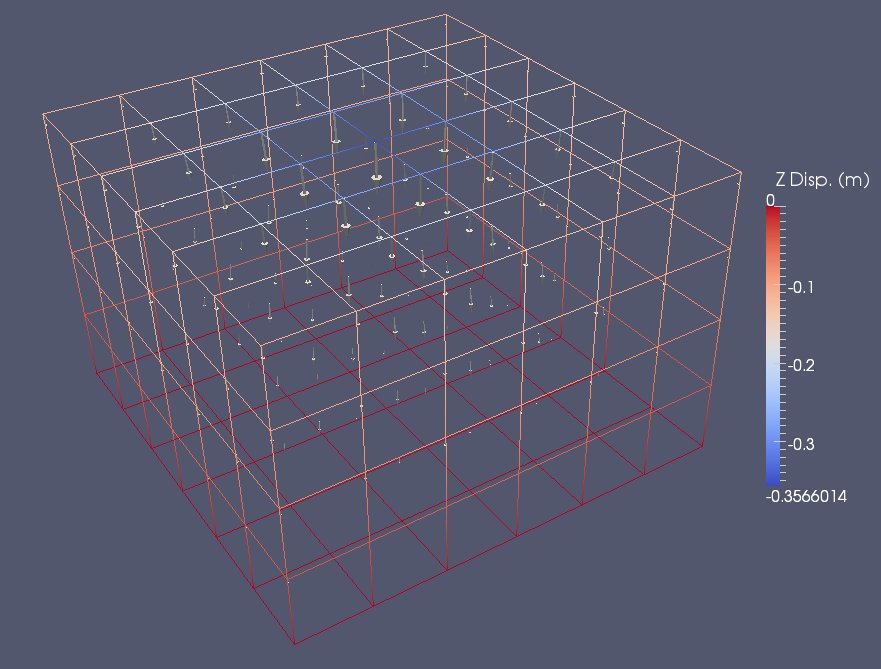
\includegraphics[width=10cm]{examples/figs/3dhex8_step18-displ}
  \caption{Displacement field for example step18 visualized using ParaView. The
    vectors show the displacement field while the colors in the wireframe
    correspond to the z-component of the displacement field.}
  \label{fig:example:3dhex8:step18:displacement}
\end{figure}


\subsubsection{Step19 - Time-Dependent Surface Load}

The \filename{step19.cfg} file defines a problem that is identical to
example step18, except that we vary the amplitude of the surface load
as a function of time. We use a temporal database (analogous to our
spatial databases for specifying spatial variations) to prescribe
a piecewise linear variation of the amplitude with time as given in
the file \filename{spatialdb/loadcycle.timedb}. The amplitude begins
at zero, progresses to 1.0, then 1.5, before decreasing in a symmetric
fashion. The temporal database can use variable time steps to prescribe
arbitrary time histories. 

Rather than specify a spatial database for the initial value of the
Neumann boundary condition corresponding to the surface load, we specify
a spatial database for the change in value and the temporal database:
\begin{cfg}[Excerpt from \filename{Step19.cfg}]
<h>[pylithapp.timedependent.bc.z_pos]</h>
<p>label</p> = face_zpos

<f>db_change</f> = spatialdata.spatialdb.SimpleDB
<p>db_change.label</p> = Amplitude of Neumann BC on +z
<p>db_change.iohandler.filename</p> = spatialdb/tractions_axial_pressure.spatialdb
<p>db_change.query_type</p> = linear ; Use linear interpolation

<f>th_change</f> = spatialdata.spatialdb.TimeHistory
<p>th_change.label</p> = Time history for Neumann BC on +z
<p>th_change.filename</p> = spatialdb/loadcycle.timedb
\end{cfg}
When we have run the simulation, the output VTK files will be contained
in \filename{examples/3d/hex8/output} (all with a prefix of \filename{step19}).
Results using ParaView are shown in Figure \vref{fig:example:3dhex8:step19:stress}.
We also output the solution at user-defined locations, which are given
in the file \filename{output\_points.txt.} See Section \vref{sec:output:points}
for a discussion of the output parameters. This type of output is
designed for comparison against observations and inversions and output
via HDF5 files (see Section \vref{sub:HDF5/Xdmf-Output}).

\begin{figure}
  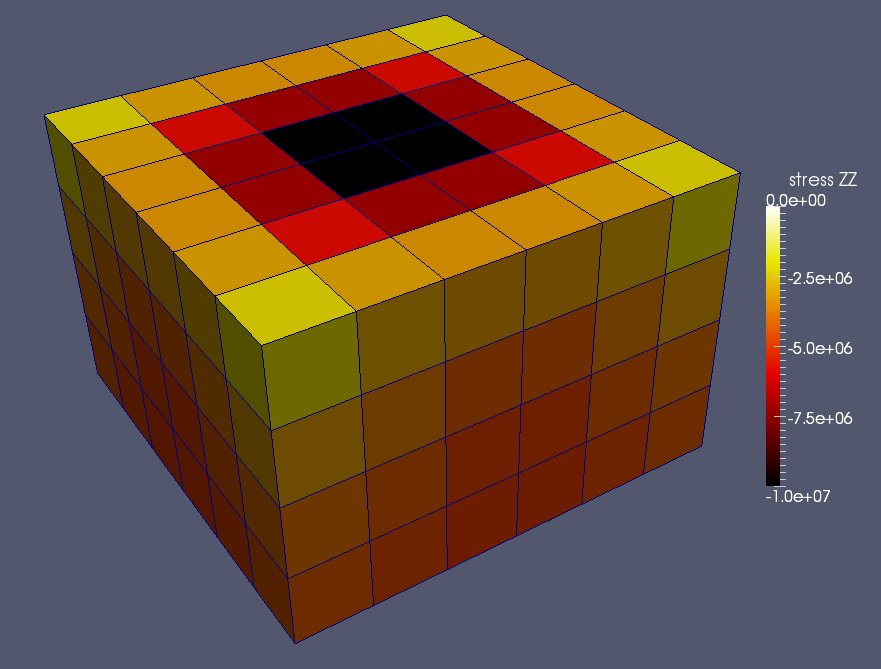
\includegraphics[width=10cm]{examples/figs/3dhex8_step19-stress_t200}
  \caption{Stress field (zz-component) for example step19 at t = 200
    years visualized using ParaView. The stresses appear as four
    layers since we have used \object{CellFilterAvg} for material
    output.}
  \label{fig:example:3dhex8:step19:stress}
\end{figure}

% End of file
